\chapter{Blockchaintoepassingen voor ERP}
\label{ch:blockchaintoepassingen-voor-erp}

Dit hoofdstuk slaat de brug tussen de twee voorgaande deelvragen. Het representeert de zoektocht naar die blockchaintechnologieën die bruikbaar zijn binnen een ERP-context. Het gaat dus over de derde deelvraag van het onderzoek:

\begin{center}
	\textit{\textbf{``Welke mogelijkheden bieden blockchains voor een ERP-systeem?''}}
\end{center}

Om die mogelijkheden te vinden, werd vertokken vanuit de Gartner Hype Cycle uit Sectie \ref{sec:verantwoording} - \nameref{sec:verantwoording}. De toepassingen blockchainplatform en \textit{smart contract} komen om die reden als eerste aan bod.

De eerste sectie geeft een inzicht in de verschillende varianten aan blockchains. Elk platform werd ontwikkeld volgens eigen ontwerpkeuzes. Als gevolg hebben ze niet allemaal hetzelfde toepassingsgebied.

De volgende sectie maakt duidelijk dat er ook scripts of programmatuur op een blockchain gebracht kunnen worden. Deze \textit{smart contracts} bieden allerlei nieuwe mogelijkheden zoals NFT's. 

Om de overstap naar de laatste deelvraag te maken, werd een laatste sectie toegeweid aan NFT's. Een concreet voorbeeld illustreert dat het mogelijk is om allerlei data in een blockchain op te nemen. Daarmee wordt een conceptuele sprong gemaakt die absoluut nodig was om de proof of concept op poten te zetten.

\section{Blockchainplatformen}

De originele \textit{Bitcoin} \textit{whitepaper} inspireerde talloze spelers om een eigen versie van een blokchain te ontwikkelen. Ondertussen brachten al verschillende ondernemingen hun eigen variant op de markt. Om deze implementaties van elkaar te onderscheiden spreekt men over verschillende ``blockchainplatformen''. Elk platform biedt een basis aan ontwikkelaars om nieuwe toepassingen te bouwen op de bestaande blokchain-infrastructuur
~\autocite{Saraf2018}.

\begin{table}[H]
	\begin{tabular}{@{}lccc@{}}
		\cmidrule(l){2-4}
		& \textbf{Ethereum}                                         & \textbf{Hyperledger} & \textbf{R3 Corda}                                        \\ \midrule
		1. Type                                                                     & Openbaar                                                  & Besloten             & Besloten                                                 \\ \midrule
		2. Consensus algoritme                                                      & Proof of Work                                             & Pluggable Framework  & Pluggable Framework                                      \\ \midrule
		3. Toepassingsgebied                                                        & Algemeen                                                  & Algemeen             & Financiële sector                                        \\ \midrule
		\begin{tabular}[c]{@{}l@{}}4. Ondersteunde\\  programmeertalen\end{tabular} & \begin{tabular}[c]{@{}c@{}}Python\\ Go\\ C++\end{tabular} & Python               & \begin{tabular}[c]{@{}c@{}}C++\\ Javascript\end{tabular} \\ \bottomrule
	\end{tabular}
	\caption{\label{tab:blockchainplatformen}Vergelijking van drie fundamentele blockchain platformen}
\end{table}

Een eerste manier waarop platformen zich van elkaar onderscheiden is de programmeertaal waarin ze geïmplementeerd zijn.
Tabel~\ref{tab:blockchainplatformen} vergelijkt drie fundamentele blockchainplatformen met elkaar op nog een aantal andere vlakken.

\begin{enumerate}
	\item Een platform kan openbaar of besloten zijn. Indien men geen permissies nodig heeft om het peer-to-peernetwerk te betreden, wordt het als openbaar beschouwd. In het andere geval is het systeem besloten. Eens een node opgevangen is in het netwerk, kan het de blockchain in beide op een transparante manier inkijken.
	\item Niet elk platform gebruikt de Proof of Work, zoals beschreven in sectie \ref{sub:proof-of-work} - \nameref{sub:proof-of-work}. Er zijn ook andere manieren om consensus na te streven. Het opzet blijft echter hetzelfde.
	\item Verschillende platformen mikken op een ander toepassingsgebied.
	\item Naast de taal waarin de blockchain geïmplementeerd is, zijn er ook programmeertalen waarmee het platform benaderd kan worden. Hiermee kunnen ontwikkelaars toepassingen schrijven die de onderliggende blockchain kunnen benutten. 
\end{enumerate}
	
\pagebreak
	
Deze drie voorbeelden werden opgenomen in de tabel, omdat ze in zekere zin een basis vormen van vele andere platformen. Heel wat producenten brachten een eigen platform op de markt dat eigenlijk een afgeleide is van reeds bestaande keuze. In de literatuur wordt vaak geen onderscheid gemaakt tussen de twee~\autocite{Gartner2022}. Enkele voorbeelden van commerciële blockchainplatformen zijn:
\begin{itemize}
	\item Ethereum
	\item Hyperledger Fabric
	\item Hyperledger Sawtooth
	\item Hyperledger Iroha
	\item IBM Blockchain
	\item Microsoft Azure Blockchain
	\item ...
\end{itemize}

\subsection{Hard forks}

Zoals reeds vermeld, kunnen blockchainplatformen de basis vormen voor nieuwe varianten. Wanneer er ingrijpende aanpassingen gemaakt worden aan het protocol van een basis-blockchain, spreekt men over een ``hard fork''. Door uiteenlopende visies kunnen op die manier verschillende ``smaken'' van eenzelfde blockchain ontstaan. Wanneer men over de Bitcoin-blockchain spreekt, heeft men het doorgaans over de originele BTC-fork. Nochtans is dit niet de enige. Sinds het ontstaan werd er steeds verder getweakt aan de implementatie. Omdat informatici een eigen visie hadden over hoe de keten stabiel gemaakt kon worden, ontstonden ook forks zoals BSV (Blockchain Satoshi Vision). In die vertakking probeerde men zoveel mogelijk terug te keren op het oorspronkelijk protocol. Verschillende ontwerpkeuzes zorgen ervoor dat de ene fork meer schaalbaarheid of rekenkracht kan bieden dan de andere. Als gevolg zijn bepaalde forks meer of minder geschikt voor het opslaan van data in een ERP-context.

\section{Smart contracts}

Een \textit{smart contract} is een stuk computercode dat geïmplementeerd wordt bovenop een blockchain als digitale versie van een contract. Ze maken het mogelijk om contractuele voorwaarden automatisch af te dwingen, zonder de tussenkomst van een derde partij~\autocite{Salem2008}.

De voorwaarden en bijhorende gevolgen van het contract, worden omgezet naar verzameling van functies en variabelen in het \textit{smart contract}. Wanneer transacties in de blockchain terecht komen die een van deze voorwaarden triggert, wordt de bijhorende functie uitgevoerd. De uitvoer wordt op zijn beurt opgenomen in de blockchain als een nieuwe transactie~\autocite{Zheng2019}. In volgende subsecties worden de verschillende stappen in de levenscyclus van een \textit{smart contract} uitgelegd. Figuur~\ref{fig:smart-contracts-overview} geeft een mooie leidraad weer.

\begin{figure}[]
	\centering
	\includegraphics[width=\linewidth]{img/blockchaintoepassingen-voor-erp/smart-contracts-overview.pdf}
	\caption{\label{fig:smart-contracts-overview}Overzicht \textit{smart contracts}~\autocite{Zheng2019}}
\end{figure}

\subsection{Creatie}

In een eerste fase leggen de betrokken partijen de voorwaarden van het contract vast in gewone mensentaal. Eens opgesteld, kan een software engineer de (voorwaarden van) dit contract omzetten in code. Dit is mogelijk in verschillende high-level programmeertalen, zoals Python, Java of Solidity~\autocite{Bahga2016}. Een compiler zet deze statements om naar een \textit{smart contract} onder de vorm machinecode, dat klaar is om in de blockchain gezet te worden~\autocite{Zheng2019}.

\textbf{Voorbeeld:}
Partijen A en B sluiten een contract: indien een metaaldetector iets aantreft in de voedselverwerking van partij A, moet partij B hiervoor beboet worden. Een software engineer krijgt de opdracht om dit contract om te zetten in code.

\subsection{Deployment}

Eens een contract wordt weggeschreven naar de blockchain, kan het niet meer gewijzigd worden. Zoals al aangegeven, zijn de voorwaarden van het contract vertaald naar functies en variabelen. Indien men een nieuwe voorwaarde wenst toe te voegen aan het contract, zal men een nieuw \textit{smart contract} moeten aanmaken. Dankzij de transparantie van de blockchain kunnen alle partijen het contract raadplegen~\autocite{Zheng2019}.

\textbf{Voorbeeld:}
Het \textit{smart contract} tussen partij A en B wordt op de blockchain geplaatst.

\subsection{Uitvoering}

Tijdens de uitvoering wordt voortdurend gemonitord of er nieuwe transacties op de blockchain geplaatst worden die de voorwaarden van het contract vervullen. Wanneer een functie getriggerd word zal deze de voorgeprogrammeerde implicaties uitvoeren als een nieuwe transactie in de blockchain. Met andere woorden: het contract werd afgedwongen, zonder actieve tussenkomst van een derde partij~\autocite{Delmolino2016}.

\textbf{Voorbeeld:}
De metaaldetector van partij A merkt een onzuiverheid op in het productieproces. Deze detectie wordt onder de vorm van een transactie opgeslagen op de blockchain. Dit triggert het \textit{smart contract} dat op zijn beurt een transactie op de keten plaatst om aan om deze gebeurtenis te documenteren.

\subsection{Afronding}

Om de levenscyclus van een \textit{smart contract} af te ronden, worden de betrokken partijen op de hoogte gebracht. De status van de partijen wordt geüpdatet indien nodig~\autocite{Zheng2019}.

\textbf{Voorbeeld:}
Partijen A en B worden op de hoogte gebracht. Partij B maakt het nodige bedrag over naar partij A, wat wordt geregistreerd als een transactie op de blockchain.



\section{NFT's}

Zoals vermeld in Subsectie \ref{sub:transacties} - \nameref{sub:transacties}, stond een transactie oorspronkelijk voor de bitcoin-overdracht van een partij naar een andere~\autocite{Pierro2017}. Bij elke transactie worden digitale tokens uitgewisseld die door de ontvangende partij opnieuw uitgegeven kunnen worden. Op geen enkel punt is het daarbij zinvol om een onderscheid te maken tussen individuele tokens. Ze zijn namelijk onderling gelijkwaardig. Zo komt een Bitcoin wallet aan zijn saldo lauter door het aantal bitcoins waaruit het bestaat. Het is daarbij niet van belang wélke bitcoin-tokens dat specifiek zijn. In die zin zijn de tokens van Blockchain 1.0 fungibel of vervangbaar.

Met de overgang naar Blockchain 2.0 wordt op dit vlak een conceptuele sprong gemaakt. Met de komst van nieuwe blockchainplatformen werd het namelijk mogelijk om meer dan enkel bitcoin-overdrachten op te slaan. De datavelden van nieuwere blockchains staan open voor allerlei data. Men kan nu ook bestanden zoals een afbeelding, factuur of tekstbestand vastleggen in een blockchain en behandelen als een token. Deze tokens kunnen nog steeds uitgewisseld worden, maar hebben nu wel een unieke waarde. Immers, de ene factuur is de andere niet. Ze zijn dus niet fungibel en krijgen daarom de naam Non-fungible token of NFT.

Een diepgaande technische uiteenzetting van NFT's is niet opportuun voor deze scriptie. Aangezien deze tokens wel hun nut bewijzen in een ERP-context, is het echter wel belangrijk om een gegrond beeld te krijgen van wat ze juist zijn.

\subsection{Voorbeeld}

Op digitale markplaatsen zoals OpenSea kan men de inhoud en details van allerlei NFT's verkennen. Deze bevinden zich op een blockchain zoals die van Ethereum. Heel wat grafische kunstwerkjes worden op die manier ``als NFT'' te koop aangeboden. Onderstaand voorbeeld illustreert wat dat juist inhoudt.

Figuur~\ref{fig:nft-example} geeft een willekeurige NFT uit de Ethereum blockchain weer, zoals die te vinden valt op digitale markplaatsen. De data die in dit geval als token op de blockchain geplaatst werd, is een PNG-afbeelding van cirkels en lijnstukken. Het is belangrijk om erop te wijzen dat dit geen afbeelding hoeft te zijn. Ook andere bestanden, zoals een XML-factuur of een mp3 zijn mogelijk. In de details wordt verwezen naar het \textit{smart contract} waarmee deze token gemaakt werd, alsook de ID dat eraan gegeven werd.

\begin{figure}[H]
	\centering
	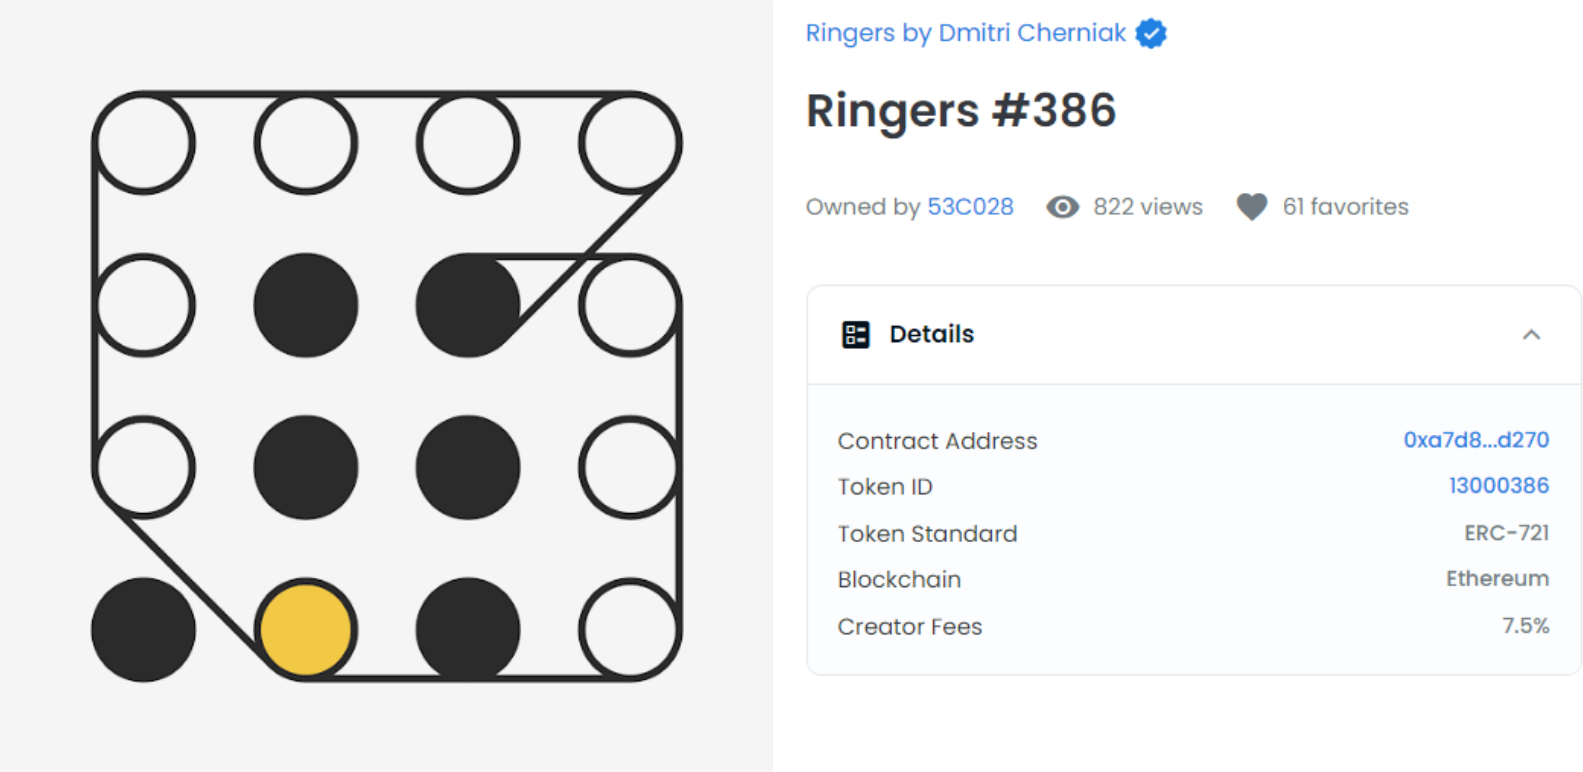
\includegraphics[width=\linewidth]{img/blockchaintoepassingen-voor-erp/nft-example.png}
	\caption{\label{fig:nft-example}NFT op een digitale marktplaats}
\end{figure}

Het \textit{smart contract} adres wijst naar een plaats op de Ethereum blockchain. Een eenvoudige manier om de bijhorende data te benaderen, is met behulp van een block explorer website zoals EtherScan. Wie het adres volgt, zal het script (of \textit{smart contract}) vinden dat gebruikt werd om de afbeelding, samen met allerlei metadata op de blockchain te plaatsen. Met andere woorden: het werd gebruikt om de afbeelding ``als NFT'' op de blockchain te plaatsen. Hiervoor heeft het script allerlei commando's. Nog een ander commando dient ervoor om de URI van een token op te vragen op basis van zijn ID:
\begin{figure}[H]
	\centering
	\includegraphics[width=\linewidth]{img/blockchaintoepassingen-voor-erp/tokenURI-function.pdf}
\end{figure}
Met de ID van de NFT uit Figuur~\ref{fig:nft-example} als parameter, zal dit commando kunnen we de bijhorende URI retourneren.

\begin{figure}[H]
	\centering
	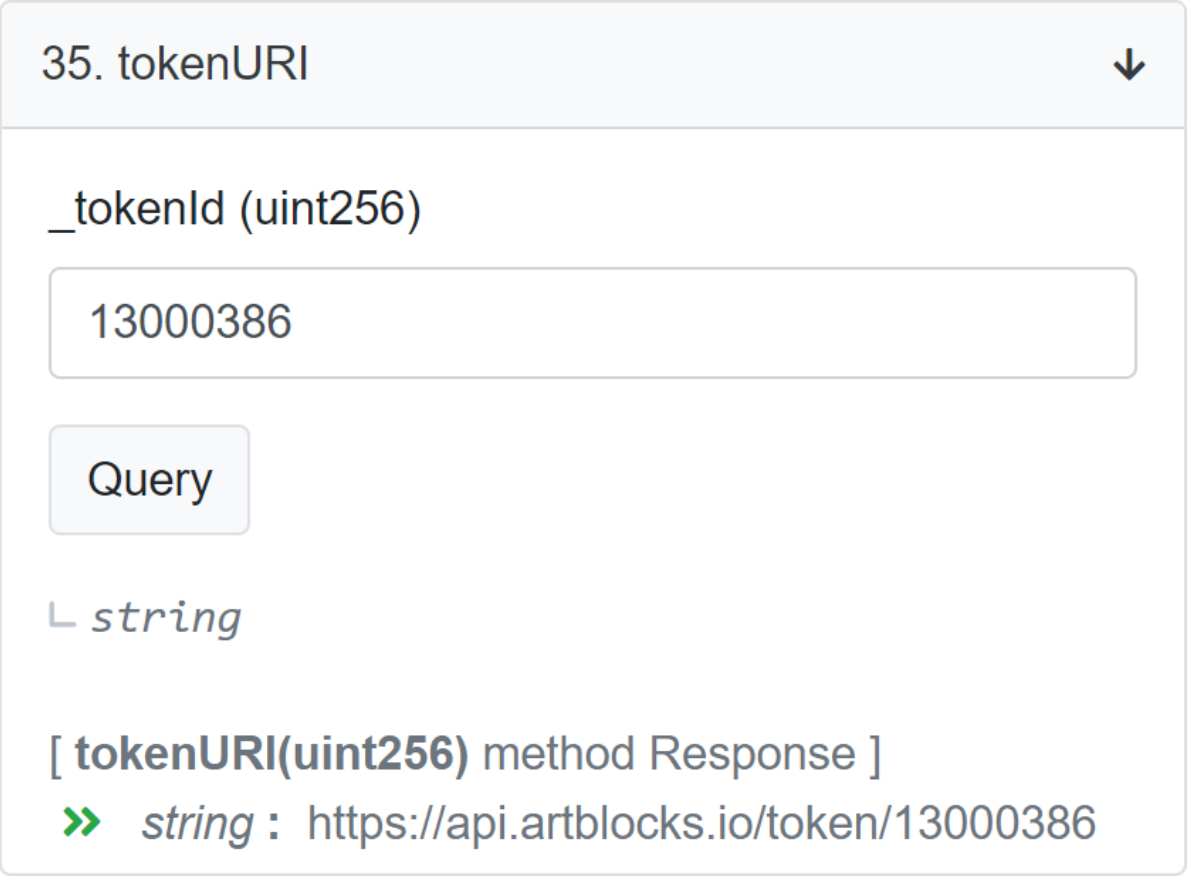
\includegraphics[width=0.5\linewidth]{img/blockchaintoepassingen-voor-erp/nft-tokenURI.png}
	\caption{\label{fig:nft-tokenURI}URI van een NFT}
\end{figure}

Merk op dat de token URI in dit geval zelfs een URL is. Deze kan dus via elke webbrowser benaderd worden. Het is trouwens ook mogelijk om dit adres als QR-code voor te stellen. Door deze verwijzing te volgen, krijgt men de data van de NFT\footnote{Voor de duidelijkheid werd een deel van de metadata uit dit voorbeeld vervangen door beletseltekens.}:

\begin{figure}[H]
	\centering
	\includegraphics[width=\linewidth]{img/blockchaintoepassingen-voor-erp/NFT-data.pdf}
\end{figure}

De NFT bestaat uit metadata zoals \verb|tokenID|, \verb*|payout_address| en \verb|minted|. Met \verb*|image| wordt de URI-verwijzing naar de PNG-afbeelding van cirkels vastgelegd. Het geheel is wat ``de NFT van'' de afbeelding inhoudt. 
Wat het betekent om een NFT van een bestand te minten kan dus eenvoudig beschreven worden: men plaatst -met behulp van een \textit{smart contract}- een URI-verwijzing naar dat bestand, samen met metadata op de blockchain. Die data geniet vanaf dan alle voordelen van een blockchain: het is \textit{incorruptible} en kan herleid worden naar een zekere eigenaar.
